
\textit{%As described in Sec.~\ref{NSP}, the research of  new resonance $X$ is one of the mail goals of LHC. With a energy achieved of 13 TeV in the center of mass and the data collected in 2016, it is possible to lead searches in a vast range of mass. One of the main final state channel in in a couple of $W^+W^-$ bosons.
In this chapter the $X \to \mathrm{W^+W^-}\to2\ell2\nu$ analysis using 2016 data is reported. To increase the sensitivity of this search, the signal must be selected in the most efficient way by reducing the
presence of the backgrounds with a similar signature: the selection criteria are described in detail. I have participated at all stages of the analysis selection (signal simulation, categorization, background estimation, etc.)  and I have been responsible for the whole analysis.} 
%The ATLAS experiment has been done this kind of searches using the early 2016 statistic, 13.2 fb$^{-1}$ and the results are shown in Fig.~\ref{ATLAS-CONF-2016-074_fig}.
%With the full 2016 statistic, approximately $\sim 36$ fb$^{-1}$ is possible to investigate a wide range of masses and, if will be no evidence of high mass signal, is possible to set  tight upper limits on the possible cross section.

\section{Overview of the fully leptonic analysis }\label{sec:AnalysisStrategy_Intro}
The analysis strategy for the high mass search in the $X \to \mathrm{W^+W^-}\to2\ell2\nu$ final state must take into account the production modes of the new scalar, the main backgrounds, and the interference among the different processes. 

The main production mode for a Higgs-like particle over the all mass spectrum is the gluon-gluon fusion process. 
However the ratio of the VBF cross-section to the gluon-gluon fusion cross-section increases with $m_\mathrm{X}$ (see Fig.~\ref{prod}), making the VBF production mechanism more and more important.\\

Among the SM processes that have the same final state of the signal or a similar one the most important are non-resonant WW production, top production, Drell-Yan. The WW production is an irreducible background and needs to be determined together with the signal in the fit. To estimate the other background processes, control regions are defined on data and compared to simulation. \\
The events are first divided according the flavour in the final state: 
\begin{itemize}
\item opposite-flavour final state, $e^{\pm} \mu^{\mp}$,
\item same-flavour final state, $e^+ e^-$ and  $\mu^+ \mu^-$. 
\end{itemize}
In the opposite-flavour final state four different jets categories are defined: the 0-jet, the 1-jet, the 2-jet and the VBF, Sec.~\ref{sec:OF}. 
In the same-flavour final state only the VBF category is considered. Indeed, only the VBF selection cuts are sufficiently tight to reduce the  overwhelming Z plus jets background to a manageable level, Sec.~\ref{sec:SF}. The jets categories improve the sensitivity of the analysis, because each category has different contributions from signal production modes and backgrounds.

The signal is interpreted in terms of the EWK singlet and MSSM models as described in Sec~\ref{NSP}. The Higgs boson width and lineshape is reweighted at generator level according to the parameters defined in the model. The interference effects between the signal produced via gluon-gluon fusion, the WW background also from gluon-gluon fusion, and SM Higgs boson, are expected to change the shape of the signal distribution and have been fully taken into account. 
A similar treatment is also applied for the interference between high mass signal produced via VBF, the WW plus two quarks background (emerging from the same initial state) and the SM Higgs generated with VBF production mechanism. In general, the interference becomes more and more important as the mass of $X$ increase and it is studied in detail in Sec~\ref{sec:signalModel}.
Finally, the interference between the $\mathrm{W^+W^-}\to2\ell2\nu$ and $\mathrm{ZZ}\to2\ell2\nu$ is negligible due to the different phase space characteristic of these processes.




\section{Main Background processes}
\label{anbkg}
Inside the SM that are several processes that have the same or a similar final state of the signal. The most important background processes contributing to this final state are non resonant $q\bar{q} \to W^+ W^-$, the top production ($t\bar{t}$ and single-top) and the Drell-Yan process. 
Other backgrounds are due to $W$+jets events, where a jet is misidentified as a lepton, and multibosons events. 
All these processes have been simulated with Monte Carlo generators and the simulation details have been discussed in Sec~\ref{MSsample}.
A detailed description of these background processes is given below:
\begin{itemize}
\item \textit{Non-resonant WW} ($q\bar{q} \to W^+ W^-$): this background is characterized by a final state identical to the signal, however the lepton kinematics for signal and $q\bar{q} \to W^+ W^-$ processes is rather different.
For the signal process, the W bosons originate from a spin-0 particle decay
and their spins must therefore be antiparallel, implying that the charged leptons produced 
in their decays appear preferentially in the same hemisphere~\cite{Ellis:2012wg}. In contrast,
there is no preferential spin direction in the background case. For this reason the
azimuthal angle difference between the two leptons is on average smaller for signal
than for background, resulting in a smaller dilepton invariant mass in the former case. The most relevant Feynman diagram of the process is shown below.
\begin{figure}[h]
\centering
\vspace{0.5cm}
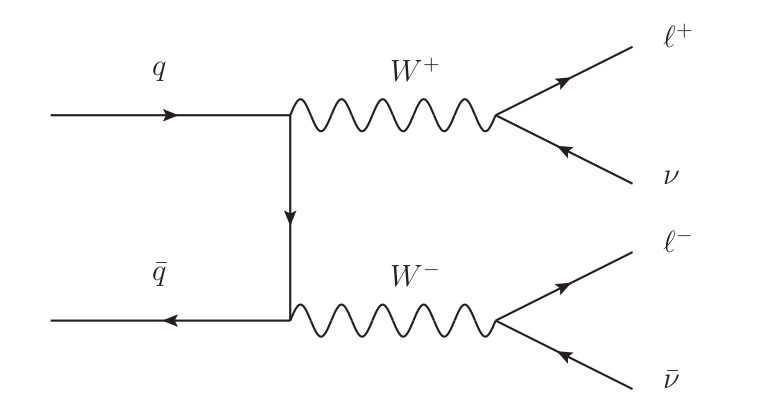
\includegraphics[scale= 0.9]{../Cap5/nnr_WW}
\end{figure}
\item \textit{Top} ($t\bar{t}$ and single-top): the $t\bar{t}$ events give a signal-like signature if both decays $t \to Wb$ are followed by $W \to \ell \nu$.  In such a case, in fact, there are two leptons and missing transverse energy,  plus two jets (from the hadronization of the $b$ quark) in the final state. This process is especially important when the signal is produced via VBS or when the signal is associated with jets coming from initial or final state radiation. The single-top production is characterized by the presence of a $W$ boson and a top quark, so after the top decay, again by two W's, but only one b-jet. Following, some examples of Feynman diagrams for the top background: the $t\bar{t}$ in (a) and (b) diagrams, the single-top in (c).
\begin{figure}[h]
\centering%
\subfigure[]%
{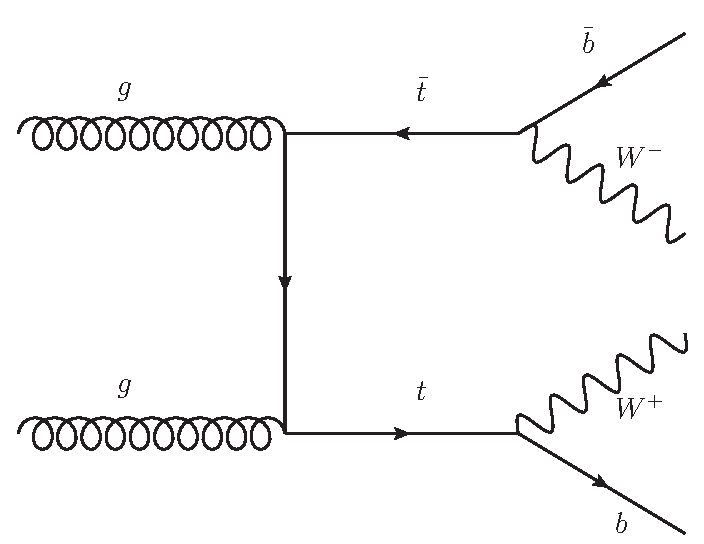
\includegraphics[scale= 0.3]{../Cap5/ggtt_t}} \qquad 
\subfigure[]%
{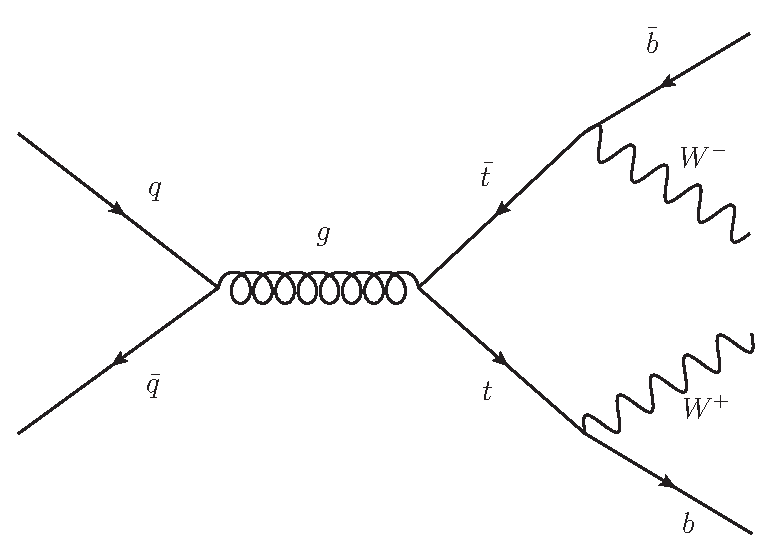
\includegraphics[scale= 0.3]{../Cap5/qqtt_s}} \qquad 
\subfigure[]%
{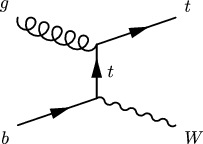
\includegraphics[scale= 0.5]{../Cap5/st_bg}}
\end{figure}
%\newpage
\item \textit{Drell-Yan}: the Drell-Yan process is defined as the annihilation of a quark-antiquark pair into a lepton-antilepton pair. This process is described at leading order by
the two  shown Feynman diagrams. %These amplitudes are proportional to the fine structure constant $\alpha \sim 1/137$.
This kind of background is particularly important for the same flavour final state of the signal
\begin{figure}[h]
\centering
\vspace{0.5cm}
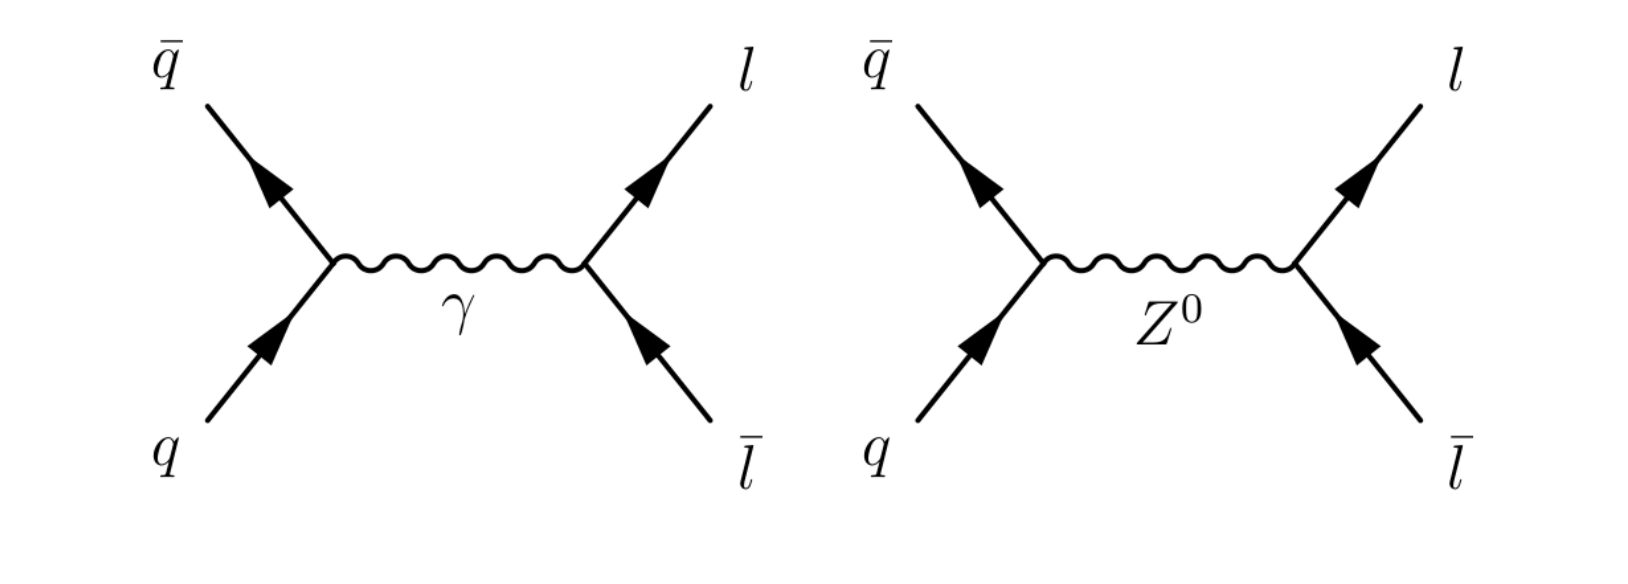
\includegraphics[scale= 0.7]{../Cap5/dy}
\end{figure}

\item \textit{W+jet}: this background is charaterized by a $W$ boson, decaying in $\ell \nu$, produced in association with a jet. If a fake lepton arise from the misidentified jet, these events have  the same final state of the signal (two leptons and missing-transverse-energy), Sec~\ref{fk}. 

\item \textit{Other}: other background processes involve multibosons production, such as $WZ/W\gamma^*$, $ZZ^*$ and $Z\gamma$ with $\gamma$ conversion.

\end{itemize}
The main background processes, the \WW production and the top production, are estimated using data. 
Instrumental backgrounds arising from non-prompt leptons in $W+$jets production and mis-measurement of $E_T^{miss}$ in Drell-Yan events are also estimated from
data. The contribution from W$\gamma^*$  is estimated partly from data. The
contribution of other sub-dominant backgrounds is obtained directly from simulated samples. The different data-driven background estimations are explained in the following sections. 
%More precisely top and  Drell-Yan backgrounds normalizations have been extracted
%directly from data-simulation comparison in specific control regions enriched in either one
%or the other background separately for the different events categories, using the rateParam feature of the combine package~\cite{combine}.


\section{Fake Lepton Background Estimation}
\label{fk}
Lepton fake rates are measured as a
function of the lepton $p_T$ and $\eta$, in a single lepton triggered sample. The test of the method and
systematic errors are described below.
In the analysis
the primary source of background from misidentification is W+Jets. QCD multi-jet and hadronic top backgrounds
are also present at much smaller level. Events in which W bosons are produced in association
with jets give rise to background to WW events when a jet is misidentified as a lepton. These
events contain a real lepton and real missing energy from the W decay. With the jet misidentified 
as a lepton, the W+Jets events have two identified leptons, missing energy, and no other
significant event characteristics. As a result, the W+Jets events cannot be easily suppressed
by event selection. This background is particularly important at low $p_T$.
The estimation of the fake lepton contribution is based on the ``fakeable object'' data-driven
method and provides a measurement of the yield and the kinematic distributions of fake background. 
It is a general technique, applicable to any physics analysis in which particle level
selection criteria are used to suppress background. The method can be used with any number
of final state particles and is independent of the event selection.
The fundamental idea of the fakeable objet method is simple: select a control sample of events
enriched in the background being estimated, and then use an extrapolation factor to relate these
events to the background in the signal region. The method is data-driven provided the control
sample is selected in data, and the extrapolation factor is measured with data. For background
arising from particle misidentification, the extrapolation is done in particle identification space
($p_T$ and $\eta$ ) of the lepton. The control sample is defined using a looser particle selection criteria
that are chosen such that the rate of misidentification is increased. The extrapolation factor
relates background misidentified with this criteria, to background misidentified as passing the
full particle selection of the signal region.



\section{Lepton Efficiencies from Tag and Probe Method}
\label{TP}
One of the well established data-driven approach for measuring the particle efficiencies is the
so called Tag and Probe method. The Tag and Probe method uses a known mass resonance (e.g. $J/\Psi$, $Z$) to select particles of the desired type, and probe the efficiency of a particular
selection criterion on these particles. In general the “tag” is an object that passes a set of very
tight selection criteria designed to isolate the required particle type. Tags are often referred
to as a “golden” electrons or muons and the fake rate for passing tag selection criteria should
be very small. A generic set of the desired particle type (i.e. with potentially very loose selection 
criteria) known as “probes” is selected by pairing these objects with tags such that the
invariant mass of the combination is consistent with the mass of the resonance. Combinatoric
backgrounds may be eliminated through any of a variety of background subtraction methods
such as fitting, or sideband subtraction. The definition of the probe objects depend on the specifics of the selection criterion being examined. The simple expression to get the efficiency %as a function of $p_T$ and $\eta$ 
is given below:
\begin{equation}
\epsilon=\frac{N_{Pass}^{Probes}}{N_{Pass}^{Probes}+N_{Fail}^{Probes}}
\end{equation}

\subsection*{Electrons} 
The   Tag and Probe is used here to get the identification and isolation efficiency of electrons. In this case, the Tag is a
well identified and isolated electron which also passes an electron trigger. 
Once the Tag electron is selected then another object that pass the kinematic electron selection, Tab.~\ref{IDe}, is searched for. 
The invariant  mass of the Tag and the Probe electron pair is reconstructed and must be in window around the Z boson mass. 
After that, to compute the efficiency, the Probe electron is required  to pass the identification tight working point. 
This procedure is performed for the data and the MC samples. 
Once data and MC efficiencies have been calculated, the electron scale factors are estimated as the ratio among the data and MC efficiencies.  
These scale factors are calculated as a function of $p_T$ and $\eta$ and used to correct the difference in efficiencies between data and MC in the analysis. 
%The Pile-Up reweighting is also applied on MC during the computation of efficiencies. 
%A MC truth matching has also been applied in case of the computation using simulation. 
%In principle, there are two methods to estimate the efficiencies.
%The first one is the \textit{counting method} and the other one is the \textit{fitting method}. 
%The counting method is used when there  are small backgrounds, instead  the fitting method instead when the backgrounds are 
%In order to take into account the effect of DY background in the efficiency estimation,  a fitting method has been used. 
%Tag and Probe pairs are  selected in Z mass window of 60 to 120 GeV.
%If there exist more than one pair then the one whose invariant mass closer to Z pole mass has been selected.
%The efficiencies have been computed as a function of $p_T$ and $\eta$ of electron.
%For signal fitting, MC templates are derived from the simulated sample in the Z mass range 60 to 120 GeV in  $p_T$ and $\eta$ bins.
%The MC Templates are then smeared using Gaussian function. For the background fitting a function, that is combination of
%an exponential function and an error function, has been used.
%The exponential decay distribution becomes
%active at high mass beyond the Z peak and the error function takes over at low masses due to
%threshold effect.
%A fit examples for all $p_T$ bins is shown in Fig.~\ref{ac}
%\begin{figure}
%\centering
%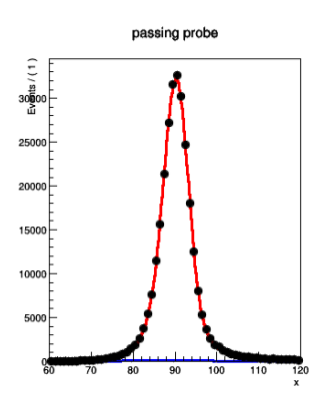
\includegraphics[scale= 0.5]{tpe}
%\caption{Fits for $p_T$ bin (35-50) GeV and $\eta$ in (-2.5,-2.0) bin.}
%\label{ac}
%\end{figure}

The electron efficiency is about 95\%, on the trigger plateau. 


\subsection*{Muons} 
The muon identification and isolation efficiency is also studied and compared to the prediction of MC in order
to understand if a correction is needed. The muon efficiency is obtained as
\begin{equation}
\epsilon_{\mu} = \epsilon_{TRK} \times \epsilon_{Tight} \times \epsilon_{ISO \; Tight} \; ,
\end{equation}
\newline
where $ \epsilon_{TRK}$ is the tracker  muon efficiency.  
The $ \epsilon_{Tight} $ is muon efficiency
under the assumption that the muon passes the kinematic selections summarized in  Tab.~\ref{IDm}.
The $\epsilon_{ISO \; Tight}$ is the efficiency of the isolation criteria under the assumption that the muon passes the same selection.
The $\epsilon_{Tight}$ and $ \epsilon_{ISO \; Tight}$ are determined  using the Tag and Probe method. 
The Tag muon is obtained by applying  the kinematic selections  and   the isolated muon trigger  with $p_T^{\mu}>20$ GeV.
The Probe muon  is requested to pass the kinematic selection and the isolation criteria.
%After that it is checked if the Probe muon is matched to the muon trigger. 
%In general the efficiencies are relatively high due to the lower cut on $p_T$ and the looser cut on
%isolation %in the double lepton trigger compared to single muon trigger. 
The efficiency value on the plateau is around 93\%-99\%.



\section{Data sample and Trigger used}

%\subsection*{Data sample}
%\subsection*{Data in CMS}
Data recorded in proton proton collisions at 13 TeV during all 2016 was used in the analysis, with a total integrated luminosity of  35.9 \fbinv.
%The data has been reprocessed in the reprocessing campaign characterized by the submission date \textit{03Feb2017} in CMS.
%In Table~\ref{tab:data} the different data streams used are presented. 
All runs are taken with a 25~ns LHC filling scheme and recorded in seven different periods, namely Run2016C, Run2016D, Run2016E, Run2016F, Run2016G, and Run2016H.
% \begin{table}
% \begin{center}
% \begin{tabular}{|l|l|}
% \hline
% Data Taking Era & Stream\\
% \hline
% \multirow{5}{*}{Run2016C} 	& SingleMuon  \\
%                                 & DoubleMuon \\
% 				& SingleElectron \\
%                                 & DoubleEG \\
% 				& MuonEG \\ \hline
% \multirow{5}{*}{Run2016D}       & SingleMuon  \\
%                                 & DoubleMuon \\
%                                 & SingleElectron \\
%                                 & DoubleEG \\
%                                 & MuonEG \\ \hline
% \multirow{5}{*}{Run2016E}       & SingleMuon  \\
%                                 & DoubleMuon \\
%                                 & SingleElectron \\
%                                 & DoubleEG \\
%                                 & MuonEG \\ \hline
% \multirow{5}{*}{Run2016F}       & SingleMuon  \\
%                                 & DoubleMuon \\
%                                 & SingleElectron \\
%                                 & DoubleEG \\
%                                 & MuonEG \\ \hline
% \multirow{5}{*}{Run2016G}       & SingleMuon  \\
%                                 & DoubleMuon \\
%                                 & SingleElectron \\
%                                 & DoubleEG \\
%                                 & MuonEG \\ \hline
% \multirow{5}{*}{Run2016H}       & SingleMuon  \\
%                                 & DoubleMuon \\
%                                 & SingleElectron \\
%                                 & DoubleEG \\
%                                 & MuonEG \\ \hline
% \hline 
% \end{tabular}
% %\vspace{0.5cm}
% \caption{Data samples used in the analysis. The total integrated luminosity corresponds to 35.9\fbinv.
% \label{tab:data}}
% \end{center}
% \end{table}


%\subsection*{Triggers path and  efficiency}
Events are required to fire one of the unprescaled single-electron, single-muon or
muon-electron triggers. Due to the rather high LHC instantaneous luminosity the
single-lepton triggers must have high HLT $p_T$ thresholds, otherwise the rate of these
triggers would be too large to be sustained. The double-lepton triggers allow the $p_T$
thresholds to be lowered while keeping a sustainable trigger rate.
%, thus maintaining a
%good sensitivity to the Higgs boson signal, for which the lepton  $p_T$ can be rather small.
The triggers used in this analysis are summarized in Table~\ref{tab:triggers}. 
%Since a final state with two leptons is searched for, both single and double lepton triggers are used. 
%For the electrons a combination of triggers is necessary to increase the statistics and to adjust the $p_T$ threshold requirement. 
\begin{table}
\begin{center}
\begin{tabular}{|l|l|}
   \hline
   Trigger name & HLT Threshold \\
   \hline
   
   SingleElectron & $p_T>$ 27 GeV  \\

   \hline
        
   SingleMuon   &  $p_T>$ 22 GeV  \\

   \hline
   
   MuonElectron       &  $p_T>$ 17 GeV  and 8 GeV  \\
   
   \hline
   
   DoubleMuon   & $p_T>$ 17 GeV  and 8 GeV  \\
      
   \hline
   
   DoubleElectron   &  $p_T>$ 23 GeV  and 12 GeV    \\
   
   \hline
\end{tabular}
\caption{Transverse momentum thresholds applied in the lepton triggers at the HLT
level. Double set of thresholds indicates the thresholds for each leg of the double lepton
triggers.}
\label{tab:triggers}  
\end{center}
\end{table}\\
\newline
The trigger efficiencies are calculated for leptons that pass the identification and isolation criteria.
In Fig.~\ref{Fig:trigger} the trigger efficiency for a gluon-gluon fusion signal with mass 300~\GeV is shown for electrons (left) and muons (right).
An average trigger efficiency greater than 99\% is found, as shown in Figure~\ref{Fig:triggerIntegral}. The triggers used in the analysis are summarized in Table~\ref{tab:triggers}. 
\begin{figure*}[htbp]
\centering
\begin{tabular}{cc}
%  \includegraphics[width=0.45\textwidth]{Figs/Trigger/ele.png} &
%  \includegraphics[width=0.45\textwidth]{Figs/Trigger/mu.png} \\
%  (a) electron & (b) muon \\
 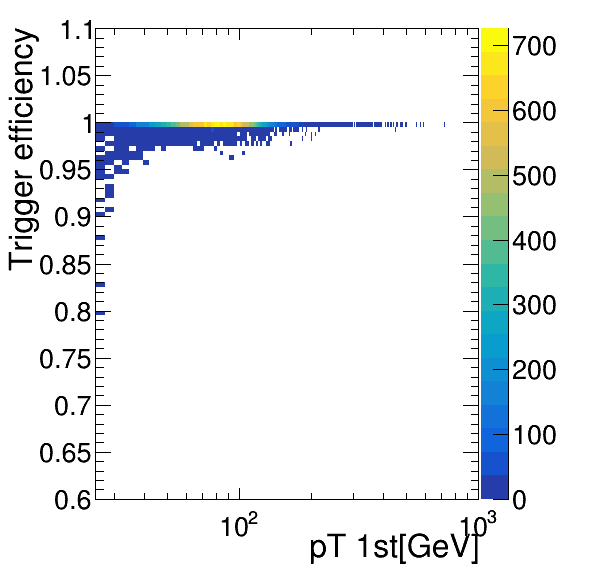
\includegraphics[width=0.45\textwidth]{../AN/Figs/Trigger/ele1.png} &
 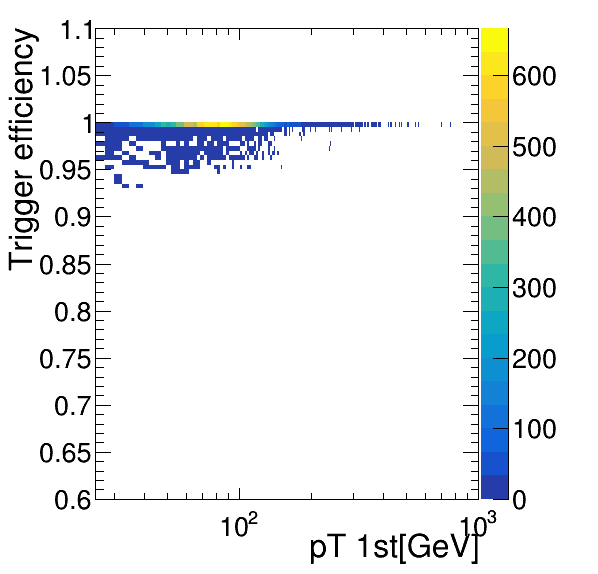
\includegraphics[width=0.45\textwidth]{../AN/Figs/Trigger/mu1.png} \\
 (a) electron 1st & (b) muon 1st \\
 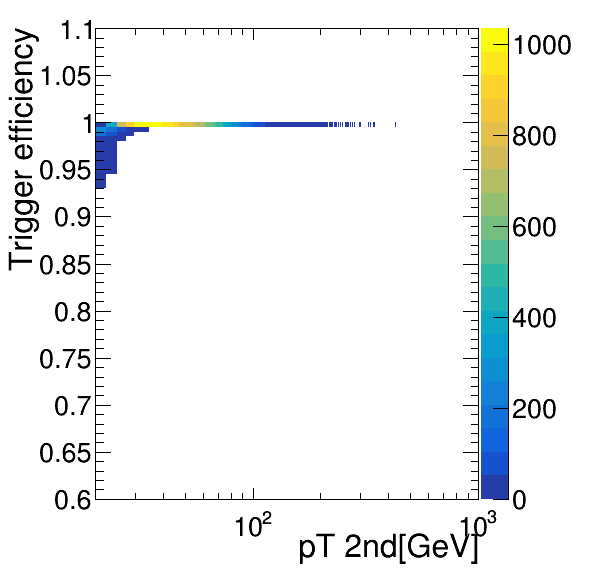
\includegraphics[width=0.45\textwidth]{../AN/Figs/Trigger/ele2.png} &
 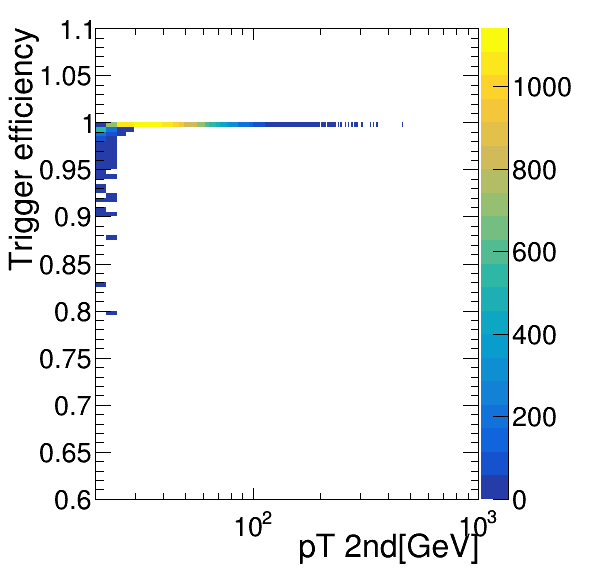
\includegraphics[width=0.45\textwidth]{../AN/Figs/Trigger/mu2.png} \\
 (c) electron 2nd & (d) muon 2nd \\
\end{tabular}
\caption{
      Trigger efficiency per event
      as a function of the lepton \pt
      for electrons (a) where leading lepton is an electron, 
      and (c) where trailing lepton is an electron, 
      and muons (b) where leading lepton is a muon, 
      and (d) where trailing lepton is an muon, 
      for a gluon fusion 300~\GeV MC sample.
      In this plots the other lepton not shown is
      integrated.
      An average trigger efficiency greater than 99\% is found.      
     }
    \label{Fig:trigger}
\end{figure*}
\begin{figure*}[htbp]
\centering
 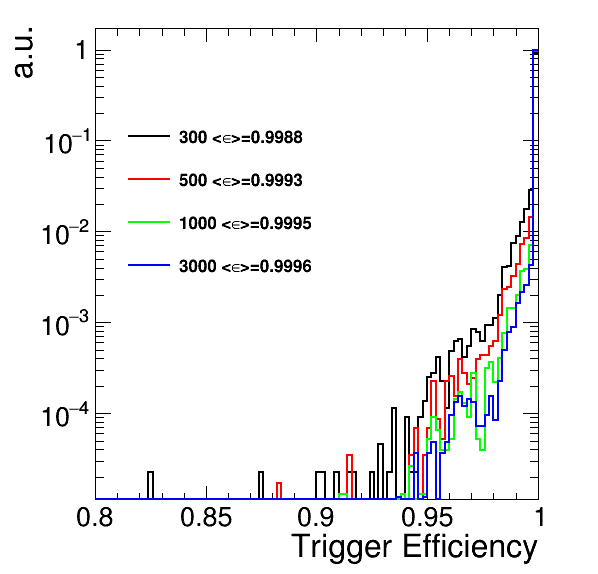
\includegraphics[width=0.6\textwidth]{../AN/Figs/Trigger/triggW.png}
\caption{
      Trigger efficiency distribution for 
      four MC samples corresponding to masses of 300, 500, 1000 and 3000~\GeV.
      An average trigger efficiency greater than 99\% is found.
     }
    \label{Fig:triggerIntegral}
\end{figure*}



\section{Discriminating variable}
This analysis is a shape analysis, meaning that after applying selection cuts, the events are not simply counted, but rather an histogram of a discriminating variable is filled from the data and fitted with the sum of signal and background templates, and finally the signal yield is extracted.
In principle, the variable with the best discriminating power would be the invariant mass of
the four lepton system, however, due to the presence of the neutrinos, it can not be measured.
Usually, in the the Higgs boson to $WW \to 2\ell 2\nu $, the variables used in the analysis are:
\begin{itemize}
\item the transverse mass, $m_T^H$, defined as,  
\begin{equation}
 m_T^H = \sqrt{2p_{\rm T}^{\ell\ell}\MET(1-\mathrm{cos}\Delta\phi(\ell\ell, \ptvecmiss))}
\end{equation}
where $\Delta\phi(\ell\ell, \ptvecmiss)$ is the azimuthal angle between the dilepton momentum and \ptvecmiss;
\item the di-lepton mass, $m_{\ell \ell}$.
\end{itemize}
However, both $m_T^H$ and $m_{\ell \ell}$, are not sensitive to different
signal mass hypothesis. For this reason a new variable, the visible transverse mass,  $m_T^I$, has been used.
This variable, studied for this specific analysis, is defined as the invariant mass of the four momentum resulting from the sum of the
two leptons four-momenta and the missing four-momentum: 
\begin{equation}
 m_T^I = \sqrt{ (p_\mathrm{\ell\ell} + \MET)^2 - (\vec{p}_\mathrm{\ell\ell} + \ptvecmiss)^2 \; .}
\end{equation}
The distribution of all the variables defined above can be compared in 
Fig.~\ref{fig:mt_nocuts}, where it is visible the better power of $m_T^I$ in discriminating different mass hypotheses wth respect to  $m_T^H$ and $m_{\ell \ell}$. The usage of  $m_T^I$ also provides a good discriminating power between signal and background.
The effects of the interference (Sec~\ref{sec:interference}) for the discriminating variable  $m_T^I$  used in the analysis is shown in Fig~\ref{nocut_mti_700_sign}
The interference is not negligible and it will take in account as part of the signal during the fit.
\begin{figure}[htbp]
\centering
\subfigure[True generated mass]{
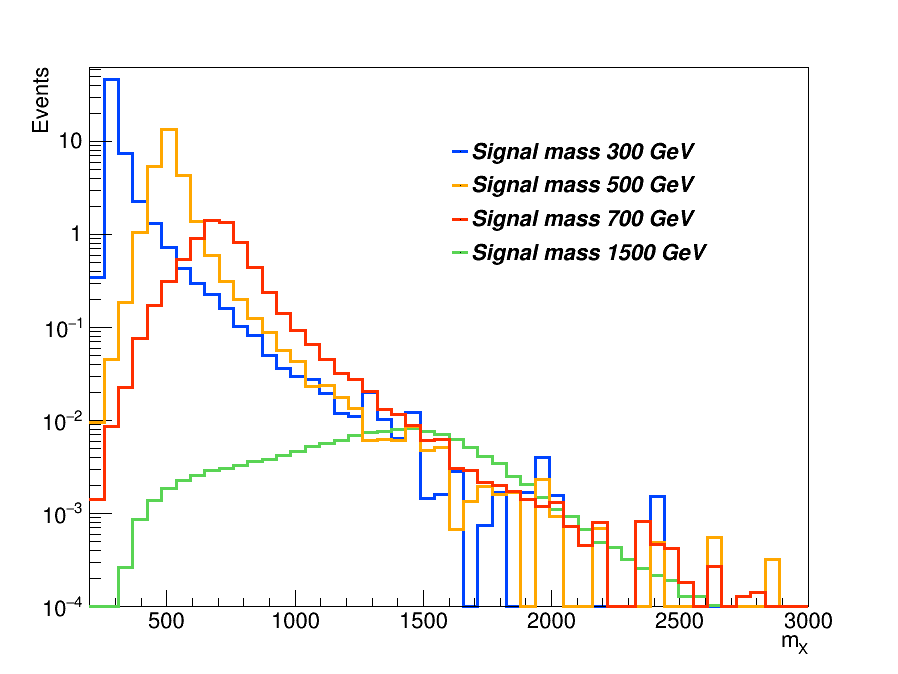
\includegraphics[width=0.45\textwidth]{../AN/Figs/Distribution_higgsLHEmass_cuts_nocuts.png}
}
\subfigure[$m_T^H$]{
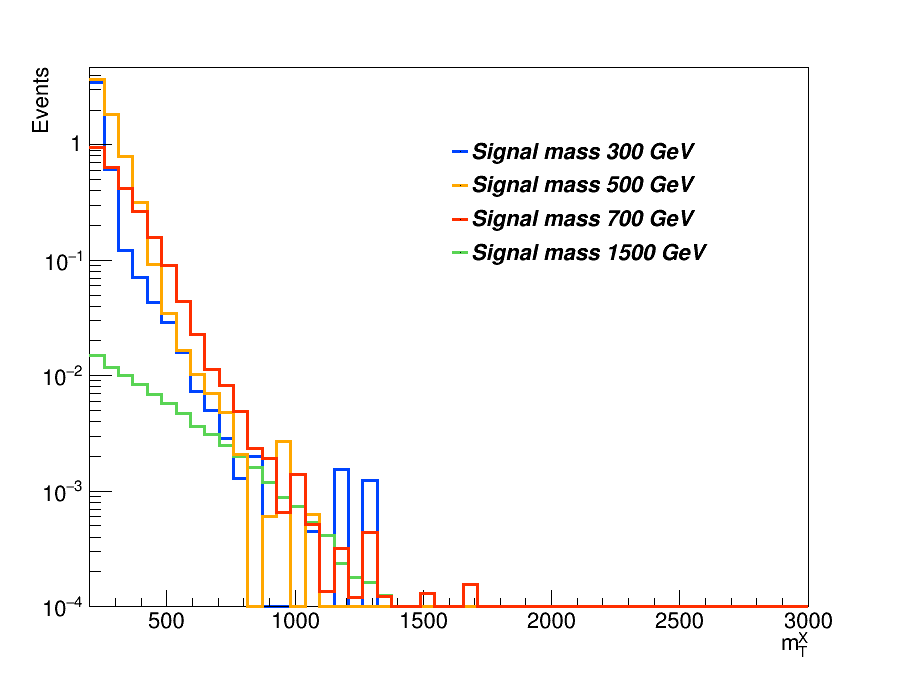
\includegraphics[width=0.45\textwidth]{../AN/Figs/Distribution_mth_cuts_nocuts.png}
}
\\
\subfigure[$m_{\ell \ell}$]{
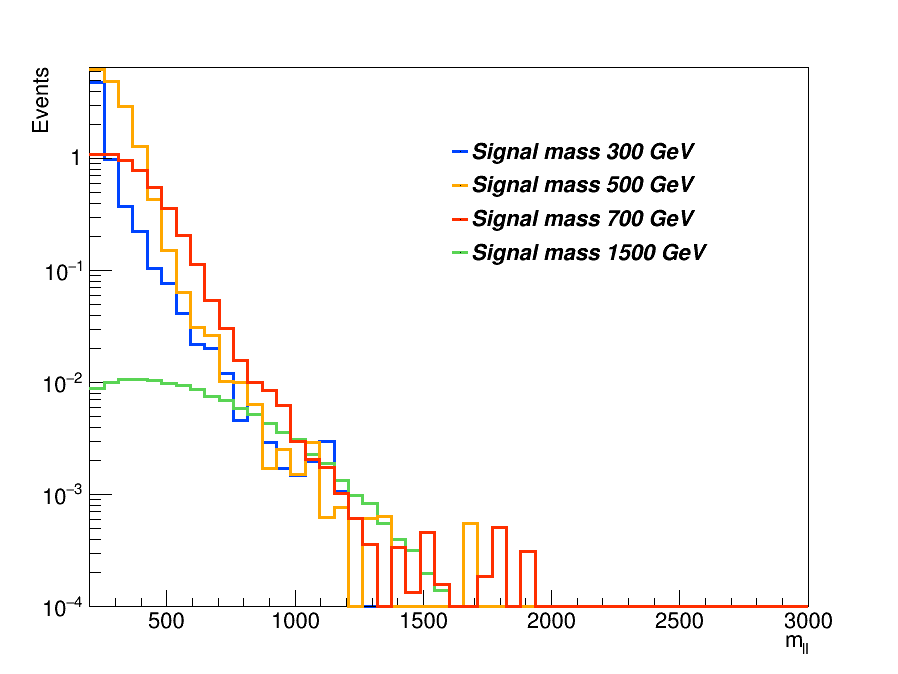
\includegraphics[width=0.45\textwidth]{../AN/Figs/Distribution_mll_cuts_nocuts.png}
}
\subfigure[$m_T^I$]{
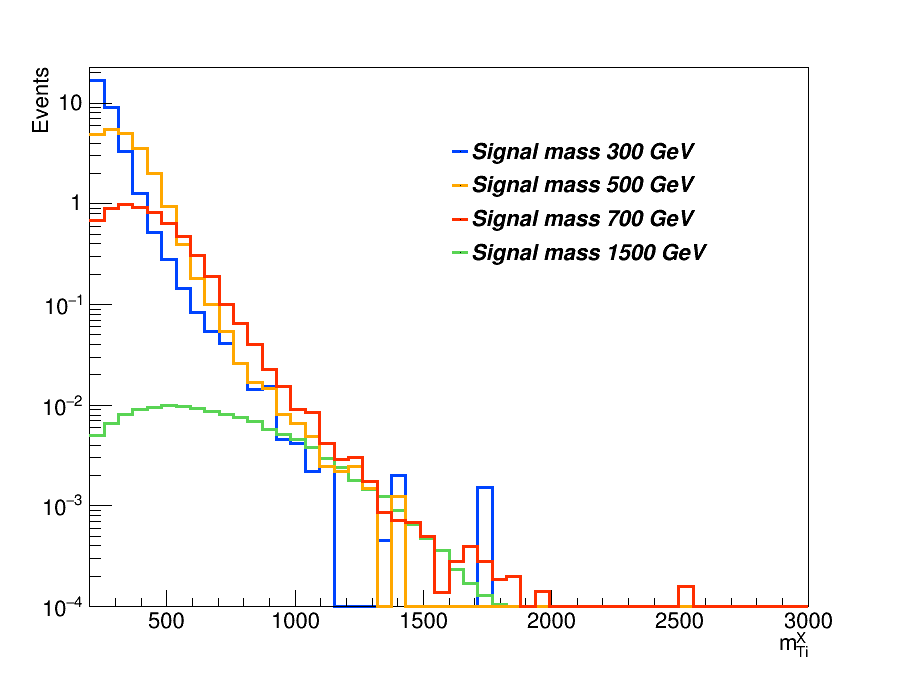
\includegraphics[width=0.45\textwidth]{../AN/Figs/Distribution_mTi_cuts_nocuts.png}
}
\caption{
    Distributions of the generated mass (no possible reconstruction), $m_T^H$, $m_{\ell \ell}$ and  $m_T^I$
    variables for different $X$ mass hypothesis. It is clear that the most discriminating variable is $m_T^I$. }
    \label{fig:mt_nocuts}
\end{figure}

\begin{figure*}[htbp]
\centering
 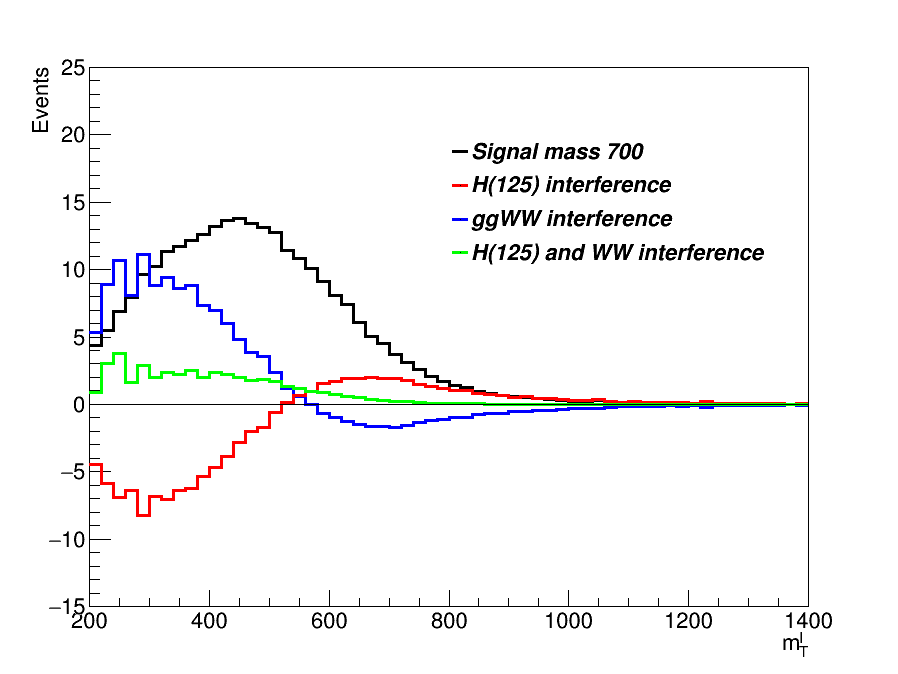
\includegraphics[width=0.6\textwidth]{../Cap5/nocut_mti_700_sign}
\caption{ The $m_T^I$ distribution at generator level for a $X$ resonances at 700 GeV produced via gluon-gluon fusion. In red the interference between the high
mass signal and the Higgs boson. In blue the interference between the high mass signal
and the background. In green the total interference i.e. high mass signal, Higgs bison and
background.       }
    \label{nocut_mti_700_sign}
\end{figure*}
